% Template setup and packages.
\documentclass[10pt,landscape,a4paper]{article}
\usepackage{multicol}
\usepackage{calc}
\usepackage{ifthen}
\usepackage{geometry}

% Custom packages.
\usepackage{amsmath}
\usepackage{mathtools}
\usepackage{amssymb}
\usepackage{mathrsfs}
\usepackage{stix2}
\usepackage{systeme}
\usepackage{graphicx}
\usepackage{float}
\usepackage{physics}
\usepackage{siunitx}
\usepackage{enumitem}
\usepackage{collcell} % loads array
\newcolumntype{M}{>{$} l <{$}}
\newcolumntype{U}{>{$[\collectcell\si} l <{\endcollectcell]$}}

% Hyperref. Remember to change title!
\usepackage{hyperref}
\hypersetup{pdfauthor={Teemu Weckroth},pdftitle={Rock Mechanics}}
%
\newcounter{Chapcounter}
\newcommand\showmycounter{\addtocounter{Chapcounter}{1}\themycounter}
\newcommand{\chapter}[1]{{\addtocounter{Chapcounter}{1}\fontsize{17}{16}\textbf{#1}}}
%
%\pagenumbering{arabic}
%\setcounter{page}{1}
%
\graphicspath{ {./figures/} }

% Change fonts for v and w.
\DeclareSymbolFont{txletters}{OML}{ntxmi}{m}{it}
\SetSymbolFont{txletters}{bold}{OML}{ntxmi}{b}{it}
\DeclareFontSubstitution{OML}{ntxmi}{m}{it}
\DeclareMathSymbol{v}{\mathalpha}{txletters}{`v}
\DeclareMathSymbol{w}{\mathalpha}{txletters}{`w}

% Commands for differentials. Redefines the underdot command!
\renewcommand\d{\mathop{}\!\mathrm{d}}
\newcommand\p{\mathop{}\!\mathrm{\partial}}

% Shrinks bullet points.
\renewcommand\labelitemi{$\vcenter{\hbox{\tiny$\bullet$}}$}

%
\ifthenelse{\lengthtest { \paperwidth = 11in}}
{ \geometry{top=.5in,left=.5in,right=.5in,bottom=.5in} }
{\ifthenelse{ \lengthtest{ \paperwidth = 297mm}}
	{\geometry{top=1cm,left=1cm,right=1cm,bottom=1cm} }
	{\geometry{top=1cm,left=1cm,right=1cm,bottom=1cm} }
}

% Turn off header and footer
\pagestyle{empty}

% Redefine section commands to use less space
\makeatletter
\renewcommand{\section}{\@startsection{section}{1}{0mm}%
	{-1ex plus -.5ex minus -.2ex}%
	{0.5ex plus .2ex}%x
	{\normalfont\large\bfseries}}
\renewcommand{\subsection}{\@startsection{subsection}{2}{0mm}%
	{-1explus -.5ex minus -.2ex}%
	{0.5ex plus .2ex}%
	{\normalfont\normalsize\bfseries}}
\renewcommand{\subsubsection}{\@startsection{subsubsection}{3}{0mm}%
	{-1ex plus -.5ex minus -.2ex}%
	{1ex plus .2ex}%
	{\normalfont\small\bfseries}}
\makeatother

% Define BibTeX command
\def\BibTeX{{\rm B\kern-.05em{\sc i\kern-.025em b}\kern-.08em
		T\kern-.1667em\lower.7ex\hbox{E}\kern-.125emX}}

% Don't print section numbers
\setcounter{secnumdepth}{0}


\setlength{\parindent}{0pt}
\setlength{\parskip}{0pt plus 0.5ex}

\begin{document}

\raggedright
\footnotesize
\begin{multicols}{3}
	% multicol parameters
	% These lengths are set only within the two main columns
	%\setlength{\columnseprule}{0.25pt}
	\setlength{\premulticols}{1pt}
	\setlength{\postmulticols}{1pt}
	\setlength{\multicolsep}{1pt}
	\setlength{\columnsep}{2pt}
	
	\part*{Rock Mechanics.}
	\begin{center}
		Teemu Weckroth, \today.
	\end{center}
	
	\section{Rock mechanics.}
	Rock mechanics aims at studying the behaviour of rocks and rock masses under loads.
	While classical mechanics deals with mechanics of non-deformable particles, rock mechanics deals with the mechanics of deformable solid bodies.
	
	\section{Units.}
	\begin{flalign*}
		\text{Length} \ [L]            & = \SI{}{\meter}                                                                                   &  \\
		\text{Area} \ [A]              & = \SI{}{\square\meter}                                                                            &  \\
		\text{Force} \ [\vb{F}]        & = \SI{}{\newton} = \SI{}{\kilogram\meter\per\square\second}                                       &  \\
		\text{Moment} \ [\vb{M}]       & = \SI{}{\newton\meter} = \SI{}{\kilogram\square\meter\per\square\second}                          &  \\
		\text{Strain} \ [\varepsilon]  & = \SI{}{-}                                                                                        &  \\
		\text{Poisson's ratio} \ [\nu] & = \SI{}{-}                                                                                        &  \\
		\text{Pressure} \ [P]          & = \SI{}{\newton\per\square\meter} = \SI{}{\pascal} = \SI{}{\kilogram\per\meter\per\square\second} &  \\
		\text{Stress} \ [\sigma]       & = \SI{}{\newton\per\square\meter} = \SI{}{\pascal} = \SI{}{\kilogram\per\meter\per\square\second} &  \\
		%				\text{Shear stress} \ [\tau]      &= \SI{}{\newton\per\square\meter} = \SI{}{\pascal} = \SI{}{\kilogram\per\meter\per\square\second} &\\
		\text{Young's modulus} \ [E]   & = \SI{}{\newton\per\square\meter} = \SI{}{\pascal} = \SI{}{\kilogram\per\meter\per\square\second} & 
	\end{flalign*}
	
	\chapter{Concepts of stress and strain.}
	
	\section{Strain in one dimension.}
	In one dimension, strain $ \varepsilon $ is defined as
	\[
		\varepsilon = \frac{\Delta L}{L_0} = \frac{L_0-L_1}{L_0}
	\]
	with length displacement $ \Delta L $, initial length of sample $ L_0 $, and final length of sample $ L_1 $.
	
	\section{Stress in one dimension.}
	In one dimension, stress $ \sigma $ is defined as
	\[
		\sigma = \frac{F}{A}
	\]
	with force $ F $ and cross-sectional area of the sample $ A $.
	
	\section{External loads.}
	\begin{flalign*}
		\text{Volume loads}       & \ \text{in} \ \SI{}{\newton\per\cubic\meter}  & \\
		\text{Surface loads}      & \ \text{in} \ \SI{}{\newton\per\square\meter} & \\
		\text{Line loads}         & \ \text{in} \ \SI{}{\newton\per\meter}        & \\
		\text{Concentrated loads} & \ \text{in} \ \SI{}{\newton}
	\end{flalign*}
	These loads are characterised by their direction, sense, and magnitude.
	
	\section{Moment.}
	The moment of a force $ \vb{F} $ (or torque) about the point $ O $ is given by
	\[
		\vb{M}_O = \vb{r} \cross \vb{F}
	\]
	and its magnitude is equal to
	\[
		M_O = Fd
	\]
	It quantifies the tendency of a force to rotate the body around a given point.
	
	\section{Global equilibrium of a body.}
	Consider a solid loaded by volume loads $ \vb{F} $, surface loads $ \vb{T} $, line loads $ \vb{Q} $, and concentrated forces $ \vb{P}_i $.
	The resulting force $ \vb{F}_0 $ must be equal to
	\[
		\vb{F}_O = \int_V{\vb{F}\d V} + \int_A{\vb{T}\d A} + \int_L{\vb{Q}\d L} + \sum_{i=1}^{m}{\vb{P}_i} = 0
	\]
	The resulting moment $ \vb{M}_O $ must be equal to
	\[
		\vb{M}_O = \int_V{\vb{x}\cross\vb{F}\d V} + \int_A{\vb{x}\cross\vb{T}\d A} + \int_L{\vb{x}\cross\vb{Q}\d L} + \sum_{i=1}^{m}{\vb{x}_i\cross\vb{P}_i} = 0
	\]
	These equations are the three equations of equilibrium in translation and the three equations of equilibrium in rotation.
	
	\section{Reactions.}
	Consider a body in equilibrium.
	It is common for such a solid to get support from the external world.
	These supports exert forces (or moments) on the body which ensures its equilibrium.
	They are called reactions.
	In general, the reactions are not known a priori.
	
	\section{Internal forces.}
	Any part of a body in equilibrium is in equilibrium.\\
	Consider a body in equilibrium under a set of external loads and reactions.
	Imagine the body to be cut in two parts L and R.
	Each part should be in equilibrium, which is not possible with external loads and reactions only.
	Therefore new forces should appear on the plane $ \pi $.
	These internal forces are due to the cohesion of matter.\\
	The internal forces which exert on both parts of a (fictive) plane are in equilibrium: $ \int{\vb{T}_R\d A} = \int{\vb{T}_L\d A} $.
	The internal forces on one side of the plane are in equilibrium with all external forces exerting from this side on the plane to the opposite side of the body.
	
	\section{Stress on a plane.}
	A force vector $ \vb{F} $ on a (real or imaginary) plane can be decomposed into a normal force $ \vb{F}_\text{n} $ acting normally to the plane and a shear force $ \vb{F}_\text{s} $ acting tangentially to the plane.
	\begin{align*}
		\vb{F}_\text{n} & =\vb{F}\cos\theta  \\
		\vb{F}_\text{s} & =\vb{F}\sin\theta 
	\end{align*}
	There are normal stresses $ \sigma_\text{n} $ and shear stresses $ \tau $ acting on the plane.
	\begin{align*}
		\sigma_\text{n}                       & =\lim_{\Delta A\rightarrow0}\frac{\Delta\vb{F}_\text{n}}{\Delta A}                                                                              \\
		\tau                                  & =\lim_{\Delta A\rightarrow0}\frac{\Delta\vb{F}_\text{s}}{\Delta A}                                                                              \\
		\text{stress vector} \ \vb{t}(\vb{x}) & =\lim_{\Delta A\rightarrow0}\left(\frac{\Delta\vb{F}}{\Delta A}\right)=\frac{\vb{\d F}}{\d A}=\begin{pmatrix}\sigma_\text{n}\\\tau\end{pmatrix}
	\end{align*}
	Consider a failure plane. The area of the failure plane is equal to
	\begin{align*}
		A'=\frac{A}{\cos\theta}
	\end{align*}
	and the normal and shear stresses on the plane are equal to
	\begin{align*}
		\sigma_\text{n} & =\frac{\vb{F}_\text{n}}{A'}=\frac{\vb{F}\cos\theta\cos\theta}{A}=\sigma_y\cos^2\theta    \\
		\tau            & =\frac{\vb{F}_\text{s}}{A'}=\frac{F\sin\theta\cos\theta}{A}=\sigma_y\sin\theta\cos\theta
	\end{align*}
	
	\section{Stress at a point (stress tensor).}
	The state of stress at any given point is defined by the force per unit area with reference to two perpendicular planes $ x $ and $ y $ through the point.\\
	In two dimensions, there are four stress components on a small square.
	\[
		\begin{pmatrix}
			\sigma_x  & \tau_{xy} \\
			\tau_{yx} & \sigma_y
		\end{pmatrix}
	\]
	In three dimensions, there are nine stress components on a small cube.
	\[
		\begin{pmatrix}
			\sigma_x  & \tau_{xy} & \tau_{xz} \\
			\tau_{yx} & \sigma_y  & \tau_{yz} \\
			\tau_{zx} & \tau_{zy} & \sigma_z
		\end{pmatrix}
	\]
	Sign convention: shear stresses are positive when they act in positive directions on negative faces.\\
	Equilibrium: to ensure that the resulting moment is equal to zero, the corresponding shear stresses should be equal $ \rightarrow $ the stress tensor is symmetrical.
	\[
		\begin{pmatrix}
			\sigma_x  & \tau_{xy} \\
			\tau_{xy} & \sigma_y
		\end{pmatrix}
	\]
	\[
		\begin{pmatrix}
			\sigma_x  & \tau_{xy} & \tau_{xz} \\
			\tau_{xy} & \sigma_y  & \tau_{yz} \\
			\tau_{xz} & \tau_{yz} & \sigma_z
		\end{pmatrix}
	\]
	The full stress transformation equations are expressed as
	\begin{align*}
		\sigma_{x'} & =\sigma_x\cos^2\theta+\sigma_y\sin^2\theta+2\tau_{xy}\sin\theta\cos\theta     \\
		\sigma_{y'} & =\sigma_x\sin^2\theta+\sigma_y\cos^2\theta-2\tau_{xy}\sin\theta\cos\theta     \\
		\tau_{x'y'} & =\tau_{xy}(\cos^2\theta-\sin^2\theta)-(\sigma_x-\sigma_y)\sin\theta\cos\theta
	\end{align*}
	\begin{figure}[H]
		\centering
		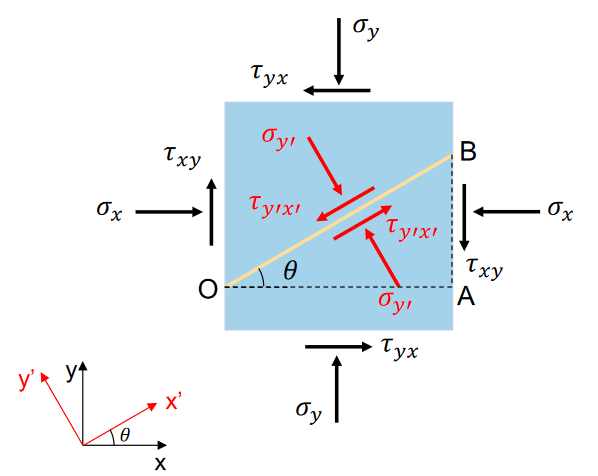
\includegraphics[width=0.18\textwidth]{stress-tensor}
	\end{figure}
	The force vector represents the same force regardless of choice of coordinate system. The same holds for the stress tensor.
	\begin{align*}
		\vb{F}                                     & =F_x\cdot\vb{e}_{\vb{x}}+F_y\cdot\vb{e}_{\vb{y}}                                                                 \\
		                                           & =F_{x'}\cdot\vb{e}_{\vb{x'}}+F_{y'}\cdot\vb{e}_{\vb{y'}}                                                         \\
		\begin{pmatrix}F_{x'}\\F_{y'}\end{pmatrix} & =\begin{pmatrix}\cos\theta&\sin\theta \\ -\sin\theta&\cos\theta\end{pmatrix}\begin{pmatrix}F_x\\F_y\end{pmatrix}
	\end{align*}
	
	\section{Principal stresses.}
	There is an inclination $ \theta^\ast $ of the axes at which all shear stresses disappear.
	The remaining stresses are principal stresses.
	\[
		\begin{vmatrix}
			\sigma_1 & 0        \\
			0        & \sigma_3
		\end{vmatrix}
	\]
	In two dimensions $ \sigma_3\leq\sigma_1 $ with minor principal stress $ \sigma_3 $ and major principal stress $ \sigma_1 $.
	\begin{align*}
		\sigma_1 & =\frac{1}{2}(\sigma_x+\sigma_y)+\sqrt{\tau_{xy}^2+\frac{1}{4}(\sigma_x-\sigma_y)^2} \\
		\sigma_3 & =\frac{1}{2}(\sigma_x+\sigma_y)-\sqrt{\tau_{xy}^2+\frac{1}{4}(\sigma_x-\sigma_y)^2}
	\end{align*}
	The orientation of the principal stresses are such that
	\[
		\tan(2\theta^\ast)=\frac{2\tau_{xy}}{\sigma_x-\sigma_y}
	\]
	Take $ \delta=\atan(\frac{2\tau_{xy}}{\sigma_x-\sigma_y}) $ with $ -\frac{\pi}{2}<\delta<\frac{\pi}{2} $.
	\[\theta^\ast=
		\begin{cases*}
			\begin{aligned}
				 & \frac{\delta}{2}               & \text{if} \ \sigma_x>\sigma_y                            \\
				 & \frac{\delta}{2}+\frac{\pi}{2} & \text{if} \ \sigma_x<\sigma_y \ \text{and} \ \tau_{xy}>0 \\
				 & \frac{\delta}{2}-\frac{\pi}{2} & \text{if} \ \sigma_x<\sigma_y \ \text{and} \ \tau_{xy}<0
			\end{aligned}
		\end{cases*}
	\]
	
	\section{Mohr circle.}
	If $ \sigma_1 $ and $ \sigma_3 $ are the principal stresses, then the state of stress on a plane inclined at an angle $ \theta $ (measured anticlockwise from $ \sigma_1 $ to the normal of the plane) is given by
	\begin{align*}
		\sigma_\text{n} & =\sigma_1\cos^2\theta+\sigma_3\sin^2\theta                                \\
		                & =\frac{1}{2}(\sigma_1+\sigma_3)+\frac{1}{2}(\sigma_1-\sigma_3)\cos2\theta \\
		\tau            & =(\sigma_1-\sigma_3)\sin\theta\cos\theta                                  \\
		                & =\frac{1}{2}(\sigma_1-\sigma_3)\sin2\theta
	\end{align*}
	The Mohr circle describes the normal and shear stresses acting on planes of all possible orientations through a stressed point in a solid.
	
	\section{Strain $ \varepsilon $ (strain tensor).}
	In one dimension, the strain at a point $x$ is found by taking the limit of an infinitesimally short bar:
	\[
		\varepsilon(x)=\lim_{L_0\to0}\frac{\Delta L}{L_0}=\lim_{\Delta x\to0}\frac{u(x+\Delta x)-u(x)}{\Delta x}=\frac{\d u}{\d x}
	\]
	Strain is essentially a measure of the relative displacement of nearby particles.\\
	Normal strains lead to change in dimensions.
	\begin{align*}
		\varepsilon_{xx}                         & =\frac{\d u_x}{\d x}                                                   \\
		\varepsilon_{yy}                         & =\frac{\d u_y}{\d y}                                                   \\
		\varepsilon_{zz}                         & =\frac{\d u_z}{\d z}                                                   \\
		\text{Volumetric strain} \ \varepsilon_V & =\frac{\Delta V}{V}=\varepsilon_{xx}+\varepsilon_{yy}+\varepsilon_{zz}
	\end{align*}
	Shear strains lead to change in angles.
	\begin{align*}
		\varepsilon_{xy} & =\frac{1}{2}\left(\frac{\d u_x}{\d y}+\frac{\d u_y}{\d x}\right)=\varepsilon_{yx} \\
		\varepsilon_{xz} & =\frac{1}{2}\left(\frac{\d u_x}{\d z}+\frac{\d u_z}{\d x}\right)=\varepsilon_{zx} \\
		\varepsilon_{yz} & =\frac{1}{2}\left(\frac{\d u_y}{\d z}+\frac{\d u_z}{\d y}\right)=\varepsilon_{zy} \\
		\gamma_{xy}      & =\frac{\d u_x}{\d y}+\frac{\d u_y}{\d x}=\alpha+\beta=\frac{1}{2}\varepsilon_{xy}
	\end{align*}
	The components of the strain tensor can be listed out in matrix form.
	\[
		\begin{pmatrix}
			\varepsilon_x    & \varepsilon_{xy} & \varepsilon_{xz} \\
			\varepsilon_{yx} & \varepsilon_y    & \varepsilon_{yz} \\
			\varepsilon_{zx} & \varepsilon_{zy} & \varepsilon_z
		\end{pmatrix}
	\]
	
	\chapter{Behaviour of rock material.}
	
	\section{Young's modulus and Poisson's ratio.}
	These parameters characterise the behaviour of the material in the elastic region.
	\begin{align*}
		\text{Young's modulus} \ E   & =\frac{\d\sigma_a}{\d\varepsilon_a}       \\
		\text{Poisson's ratio} \ \nu & =-\frac{\d\varepsilon_r}{\d\varepsilon_a}
	\end{align*}
	
	\section{Unconfined (uniaxial) compression test.}
	Measured quantities:
	\begin{itemize}
		\item Axial compressive load $F$
		\item Change in measured axial length $\Delta l$
		\item Change in radius $\Delta r$
	\end{itemize}
	Transformed quantities:
	\begin{itemize}
		\item Axial stress $\sigma_a=\frac{F}{A_0}$
		\item Axial strain $\varepsilon_a=\frac{\Delta l}{l_0}$
		\item Radial strain $\varepsilon_r=\frac{\Delta r}{r_0}$
	\end{itemize}
	Stress-strain curve:
	\begin{enumerate}[label=\Roman*.]
		\item Initial portion of the curve, concave upwards. Closing of initial micro-cracks.
		\item Linear elastic behaviour (both axially and radially).
		\item The axial stress-strain curve is nearly elastic. Significant acoustic emissions corresponding to an increase in micro-cracking can be recorded.
		\item The rock has undergone a rapid acceleration of micro-cracking events and volume increases.
		\item Post-peak domain.
	\end{enumerate}
	\begin{align*}
		\text{Peak strength} & = \text{Uniaxial compressive strength} = \sigma_c          \\
		                     & = \text{Maximum strength that a rock specimen can sustain} \\
		                     & \quad \ \text{under a given set of conditions}
	\end{align*}
	\begin{figure}[H]
		\centering
		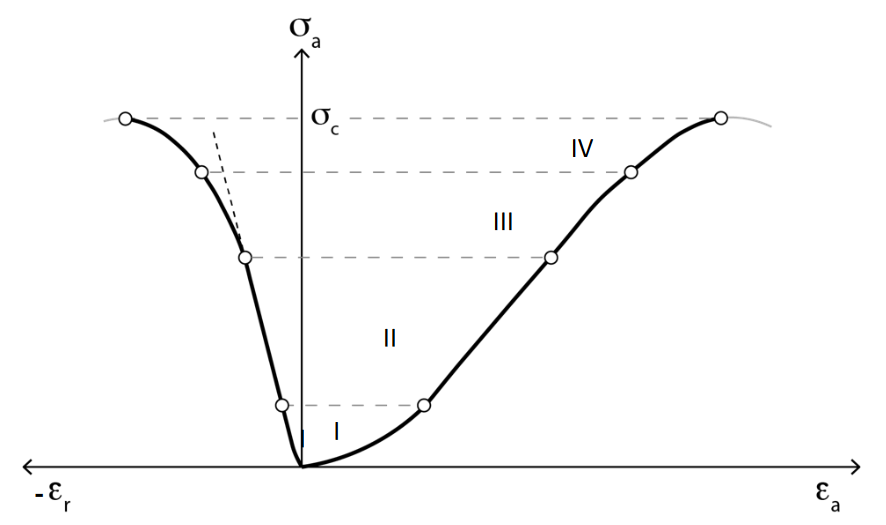
\includegraphics[width=0.25\textwidth]{unconfined-uniaxial}
	\end{figure}
	\begin{table}[H]\scriptsize\centering\begin{tabular}{l c c}
			Rock material         & $E \ (\SI{}{\giga\pascal})$ & $\sigma_c \ (\SI{}{\mega\pascal})$ \\
			\hline
			Chalk                 & \SIrange{0.1}{12}{}         & \SIrange{0.1}{12}{}                \\
			Coal                  & \SIrange{1}{6}{}            & \SIrange{2}{100}{}                 \\
			Sandstone (soft)      & \SIrange{1}{10}{}           & \SIrange{1}{10}{}                  \\
			Limestone (very soft) & \SIrange{3}{10}{}           & \SIrange{2}{10}{}                  \\
			Shale                 & \SIrange{10}{70}{}          & \SIrange{10}{70}{}                 \\
			Sandstone(hard)       & \SIrange{20}{80}{}          & \SIrange{20}{80}{}                 \\
			Limestone (very hard) & \SIrange{50}{100}{}         & \SIrange{100}{300}{}               \\
			Basalt                & \SIrange{35}{100}{}         & \SIrange{60}{350}{}
		\end{tabular}\end{table}
	Rocks generally fail at a small strain, typically around $\SIrange{0.2}{0.4}{\percent}$.
	Brittle rocks (typically crystalline rocks) have low strain at failure while soft rocks (e.g. shale and mudstone) tend to have relatively high strain at failure.
	Most rocks exhibit brittle behaviour under uniaxial compression.
	
	\section{Failure.}
	Strength in rock mechanics is defined as the peak stress a material can sustain (at failure.)
	However, the compression test does not have to end in rupture at that point but may proceed all the way to point $R$.
	
	\section{Confining stress.}
	At depth, rock is subjected to axial and lateral stresses.
	True triaxial compression means three different principal stresses.
	It is often simplified by making two lateral stresses equal to minor principal stress.\\
	The behaviour of rock in triaxial compression changes with increasing confining pressure:
	\begin{itemize}
		\item Peak strength increases.
		\item Post-peak behaviour from brittle gradually changes to ductile.
	\end{itemize}
	Stress-strain behaviour at elastic region appears the same as uniaxial compression.\\
	Brittle to ductile transition:\\
	\begin{table}[H]\scriptsize\centering\begin{tabular}{l c}
			Rock type & Confining pressure $\SI{}{\mega\pascal}$ \\
			\hline
			Rock salt & $0$                                      \\
			Chalk     & $<10$                                    \\
			Shale     & $\SIrange{0}{20}{}$                      \\
			Limestone & $\SIrange{20}{100}{}$                    \\
			Sandstone & $>100$                                   \\
			Granite   & $>>100$

			
		\end{tabular}\end{table}
	
	\section{Failure criteria.}
	A failure criterion is a hypothesis concerning the stress at failure under any combination of stresses.
	It is an equation that links the stress components which will permit to predict the peak strengths developed under various stress combinations.
	It typically takes one of the following forms:
	\begin{align*}
		\sigma_1 & =f(\sigma_2,\sigma_3) \\
		\tau     & =f(\sigma_\text{n})
	\end{align*}
	
	\section{Mohr-Coulomb criterion.}
	According to the Mohr-Coulomb criterion, the shear strength is made up of two parts:
	\[
		\tau=c+\sigma_\text{n}\tan\phi,
	\]
	where $c$ is a constant cohesion and $\sigma_\text{n}\tan\phi$ is a frictional component.\\
	It is a straight line with an intercept $c$ on the $\tau$-axis and an angle $\phi$ with the $\sigma_\text{n}$-axis.\\
	The criterion assumes that a shear failure plane is developed in the rock material.
	When failure occurs, the stresses developed on the failure plane are on the failure criterion.\\
	In the $\sigma_\text{n}$-$\tau$ diagram, when the Mohr circle touches the Mohr-Coulomb strength envelope, the stress condition on the failure plane meets the strength criterion.
	\begin{figure}[H]
		\centering
		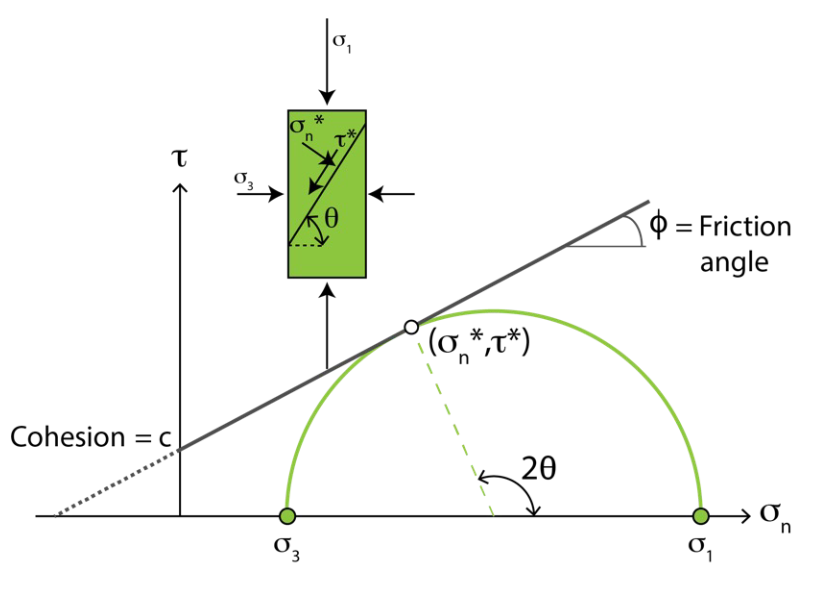
\includegraphics[width=0.25\textwidth]{mohr-coulomb-criterion}
	\end{figure}
	Express $\sigma_n$ and $\tau$ as functions of $\sigma_1$ and $\sigma_3$:
	\begin{align*}
		\sigma_n & =\frac{1}{2}(\sigma_1+\sigma_3)+\frac{1}{2}(\sigma_1-\sigma_3)\cos2\theta \\
		\tau     & =\frac{1}{2}(\sigma_1-\sigma_3)\sin2\theta
	\end{align*}
	Rearranging
	\[
		\frac{1}{2}(\sigma_1-\sigma_3)\sin2\theta=c+\left[\frac{1}{2}(\sigma_1+\sigma_3)+\frac{1}{2}(\sigma_1-\sigma_3)\cos2\theta\right]\tan\phi
	\]
	gives
	\[
		\sigma_1=\frac{2c+\sigma_3(\sin2\theta+\tan\phi(1-\cos2\theta))}{\sin2\theta-\tan\phi(1+\cos2\theta)}
	\]
	The Mohr circle construction gives the orientation of the failure plane:
	\[
		\theta=\frac{\pi}{4}+\frac{\phi}{2}
	\]
	For the failure plane
	\[
		\sin 2\theta=\cos\phi \qquad \cos2\theta=-\sin\phi
	\]
	so the Mohr-Coulomb criterion can be written as
	\begin{align*}
		\sigma_1 & =\frac{2c\cos\phi+\sigma_3(1+\sin\phi)}{1-\sin\phi}=\frac{2c\cos\phi}{1-\sin\phi}+\sigma_3\frac{1+\sin\phi}{1-\sin\phi} \\
		         & =\sigma_c+\sigma_3\tan\psi
	\end{align*}
	According to the Mohr-Coulomb criterion, failure occurs when the applied shear stress minus the frictional resistance related to the normal stress on the failure plane
	\[
		\tau-\sigma_\text{n}\tan\phi=c
	\]
	becomes equal to the rock cohesion.\\
	The Mohr-Coulomb criterion has no physical meaning in presence of tensile normal stress. However, the Mohr-Coulomb criterion is often extrapolated into the tensile region until the tensile strength is reached.
	
	\section{Tensile cut-off.}
	Actual rock tensile strengths $\sigma_t$ are lower than predicted by the Mohr-Coulomb criterion $\sigma_{t(MC)}$.
	A tensile cut-off is usually applied at a selected value of uniaxial tensile stress $\sigma_t=-T_0$ (at about $1/10\sigma_c$).
	
	\section{Hoek-Brown criterion.}
	The Mohr-Coulomb criterion is only suitable for the low range of confining stress.
	At high confining stress, it overestimates the strength.
	Therefore, a number of empirical strength criteria have been introduced for practical use.
	One of the most widely used criteria is the Hoek-Brown criterion of isotropic rock materials.
	The Hoek-Brown criterion is expressed as
	\[
		\sigma_1=\sigma_3+(m\sigma_c\sigma_3+\sigma_c^2)^{0.5}
	\]
	with $m$ a parameter that changes with rock type (usually between $5$ and $30$).
	The Hoek-Brown strength envelope is a curve.
	At high stress level, the envelope curves down.
	It gives a lower strength estimate that the Mohr-Coulomb criterion.
	
	\section{Effect of specimen size.}
	Both compressive strength and the brittleness are reduced for larger specimens.
	The elastic modulus does not vary significantly with specimen size.
	The larger the specimen, the greater the number of micro-cracks and hence the greater the likelihood of a more severe flaw.
	
	\section{Effect of specimen dimensions (constant $V$).}
	The elastic modulus does not vary significantly with specimen dimensions.
	Both the strength and the ductility increase as the aspect ratio (ratio of diameter to length) increases (effect of steel platens restraining deformation of the specimen).
	
	\section{Effect of water.}
	Deformation and failure of are controlled by the effective stresses
	\[
		\sigma'=\sigma-p_wI
	\]
	Deformability, compressive strength, and the post-peak behaviour of some rocks (especially those with a high clay mineral content) are affected by the moisture content.
	\begin{itemize}
		\item Desiccation (the rock becomes more friable)
		\item Swelling phenomena
		\item Slaking phenomena (the rock can break down and crumble)
	\end{itemize}
	
	\section{Effect of temperature.}
	Increase in temperature reduces the elastic modulus and compressive strength.
	Increase in temperature increases the ductility in the post-peak region.
	
	\section{Effect of pore fluid pressure.}
	Rocks are porous materials, and the pore space of a rock will in situ be filled with fluids under pressure.
	Deformation and failure of are controlled by the effective stresses
	\[
		\sigma_1'=\sigma_1-p \qquad \sigma_2'=\sigma_2-p \qquad \sigma_3'=\sigma_3-p
	\]
	where $p$ is the pore fluid pressure.\\
	Shear stresses are not affected by pore fluid pressure!\\
	A pore fluid pressure $p$ causes the same reduction in peak strength as a reduction of the external total pressure by an amount equal to $p$.\\
	The effect of pore fluid pressure can be input in the failure criteria simply by restating the conditions for failure in terms of effective stresses
	\begin{align*}
		\text{Mohr-Coulomb criterion} \ \sigma_1' & =\sigma_c+\sigma_3'\tan\psi                      \\
		\text{Hoek-Brown criterion} \ \sigma_1'   & =\sigma_3'+(m\sigma_c\sigma_3'+\sigma_c^2)^{0.5}
	\end{align*}
	In the context of a Mohr diagram, replacing the stresses $\sigma_i$ with the effective stresses $\sigma_i'$ has the effect of translating all the stress circles to the left by the amount $p$.
	
	\chapter{Underground excavations.}
	
	\section{Types of underground excavations.}
	Underground excavation is a general term.
	It includes
	\begin{itemize}
		\item boreholes for water, hydrocarbon, or geothermal energy extraction (small diameter; vertical, horizontal, or inclined)
		\item shafts for mine or tunnel access (large diameter; vertical)
		\item tunnels for highways and railroads (large diameter; horizontal)
		\item caverns for hydroelectric power production and storage of water, oil, liquefied natural gas... (specific and non-circular geometries; large size; cyclic loading)
		\item caverns for mining purposes (intended to be stable while the ore is removed; or intentionally collapsed to produce broken rock that is drawn off as the ground caves)
	\end{itemize}
	The underground site is usually inaccessible until actual construction.
	The rock is initially stressed - the excavation causes changes in the stress state.
	
	\section{Problem description.}
	Consider a 2D cross-section.
	$\sigma_{x0}$ and $\sigma_{y0}$ are the (far-field) principal stresses.
	It is convenient to work with cylindrical system of coordinates.
	Define the normal stresses:
	\begin{align*}
		\text{radial stress} \ \sigma_r \\
		\text{hoop stress} \ \sigma_\theta
	\end{align*}
	Define the shear stress:
	\[
		\tau_{r\theta}=\tau_{\theta r}
	\]
	\begin{figure}[H]
		\centering
		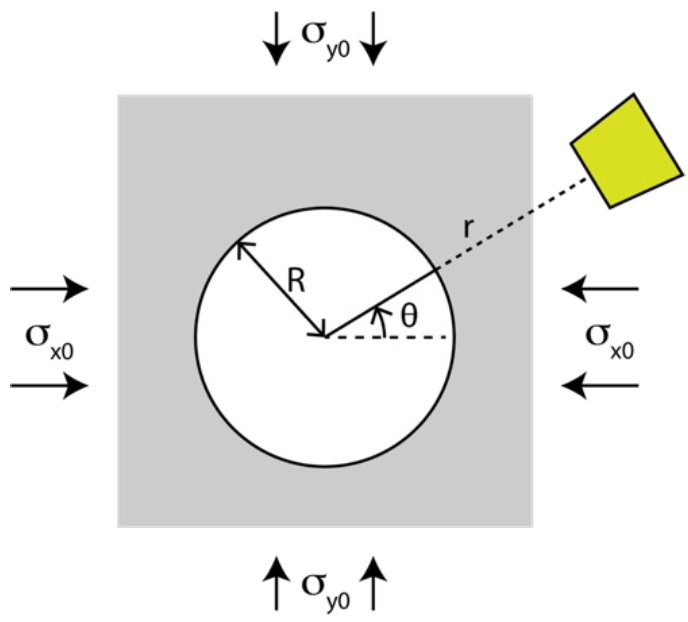
\includegraphics[width=0.11\textwidth]{kirsch-analytical}
	\end{figure}
	
	\section{Kirsch analytical solution.}
	The Kirsch solution is the solution to the problem of a circular hole in a bi-axially loaded plate of homogeneous, isotropic, continuous, and linearly elastic material.
	It can be assimilated to a tunnel, well, or shaft which is sufficiently deep to neglect changes in state of stress around the zone of interest.\\
	%		$\sigma_r$ is the radial stress, $\sigma_\theta$ is the hoop (also known as orthoradial, tangent, or circumferential) stress, and $\tau_{r\theta}=\tau_{\theta r}$ is the shear stress.\\
	The elastic stress field around a circular opening is given by
	\begin{align*}
		\sigma_r       & = \frac{\sigma_{x0}+\sigma_{y0}}{2}\left(1-\frac{R^2}{r^2}\right) + \frac{\sigma_{x0}-\sigma_{y0}}{2}\left(1-\frac{4R^2}{r^2}+\frac{3R^4}{r^4}\right)\cos2\theta \\
		\sigma_\theta  & = \frac{\sigma_{x0}+\sigma_{y0}}{2}\left(1+\frac{R^2}{r^2}\right) - \frac{\sigma_{x0}-\sigma_{y0}}{2}\left(1+\frac{3R^4}{r^4}\right)\cos2\theta                  \\
		\tau_{r\theta} & = -\frac{\sigma_{x0}-\sigma_{y0}}{2}\left(1+\frac{2R^2}{r^2}-\frac{3R^4}{r^4}\right)\sin2\theta
	\end{align*}
	With the lateral earth pressure coefficient $K=\frac{\sigma_{x0}}{\sigma_{y0}}$
	\begin{align*}
		\sigma_r       & = \frac{\sigma_{y0}(K+1)}{2}\left(1-\frac{R^2}{r^2}\right) + \frac{\sigma_{y0}(K-1)}{2}\left(1-\frac{4R^2}{r^2}+\frac{3R^4}{r^4}\right)\cos2\theta \\
		\sigma_\theta  & = \frac{\sigma_{y0}(K+1)}{2}\left(1+\frac{R^2}{r^2}\right) - \frac{\sigma_{y0}(K-1)}{2}\left(1+\frac{3R^4}{r^4}\right)\cos2\theta                  \\
		\tau_{r\theta} & = -\frac{\sigma_{y0}(K-1)}{2}\left(1+\frac{2R^2}{r^2}-\frac{3R^4}{r^4}\right)\sin2\theta
	\end{align*}
	and
	\begin{align*}
		\frac{\sigma_r}{\sigma_{y0}}       & = \frac{K+1}{2}\left(1-\frac{R^2}{r^2}\right) + \frac{K-1}{2}\left(1-\frac{4R^2}{r^2}+\frac{3R^4}{r^4}\right)\cos2\theta \\
		\frac{\sigma_\theta}{\sigma_{y0}}  & = \frac{K+1}{2}\left(1+\frac{R^2}{r^2}\right) - \frac{K-1}{2}\left(1+\frac{3R^4}{r^4}\right)\cos2\theta                  \\
		\frac{\tau_{r\theta}}{\sigma_{y0}} & = -\frac{K-1}{2}\left(1+\frac{2R^2}{r^2}-\frac{3R^4}{r^4}\right)\sin2\theta
	\end{align*}
	
	\section{Stress field for isotropic stress states ($K=1$).}
	The stress field around a circular opening is given by
	\begin{figure}[H]
		\centering
		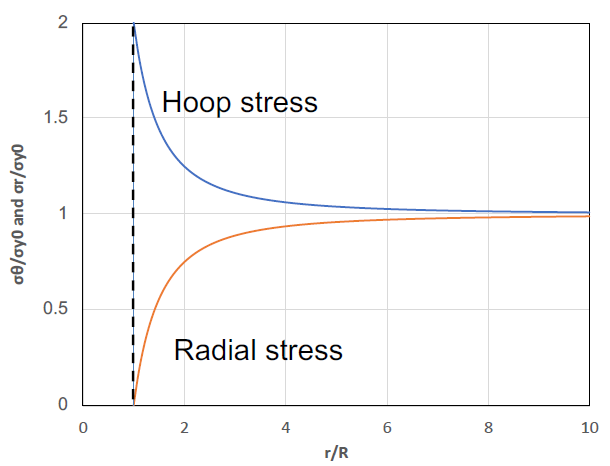
\includegraphics[width=0.16\textwidth]{stress-field}
	\end{figure}
	The opening alters the pre-existing states of stress.
	%\begin{figure}[H]
	%	\centering
	%	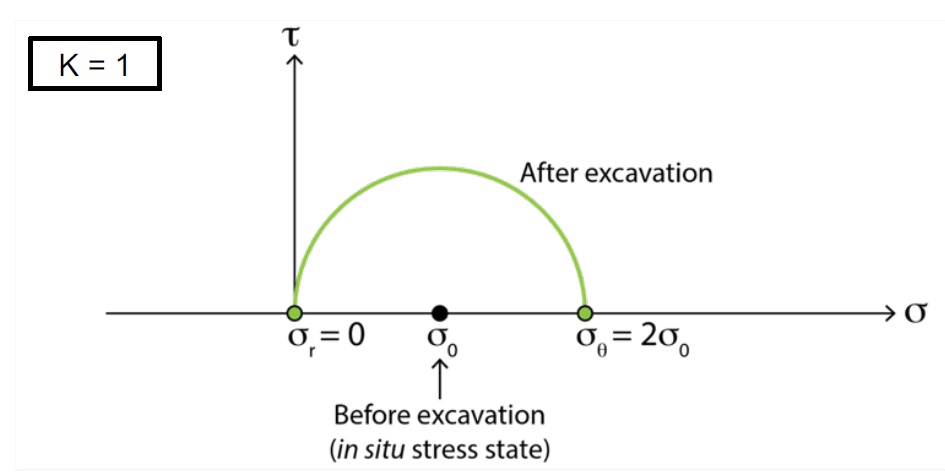
\includegraphics[width=0.25\textwidth]{stress-field-mohr}
	%\end{figure}
	
	\section{Stresses at the boundary of a circular opening.}
	For $r=R$, the Kirsch equations yield
	\begin{align*}
		\sigma_r      & = 0 \ \text{(no internal pressure)}                             \\
		\sigma_\theta & = \sigma_{x0}+\sigma_{y0}-2(\sigma_{x0}-\sigma_{y0})\cos2\theta
	\end{align*}
	or, if $\sigma_{x0}=K\sigma_{y0}$
	\begin{align*}
		\sigma_\theta  & = \sigma_{y0}\left[(1+K)+2(1-K)\cos2\theta\right]                     \\
		\tau_{r\theta} & = 0 \ \text{(as the excavation boundary is a principal stress plane)}
	\end{align*}
	\begin{enumerate}[label=(\alph*)]
		\item Under all stress fields, the opening alters the pre-existing state of stress (stress concentrations)
		\item There is a linear variation with $K$ of these stress concentrations
		\item For an isotropic stress field ($K=1$), the stress concentration is $2$ everywhere on the boundary
		\item In a uniaxial stress field ($K=0$), the maximum stress concentration is $3$ (compressive) and the minimum stress concentration is $-1$ (tensile)
		\item Tension on the boundary can occur if $K<\frac{1}{3}$ (or $>3$)
	\end{enumerate}
	\begin{figure}[H]
		\centering
		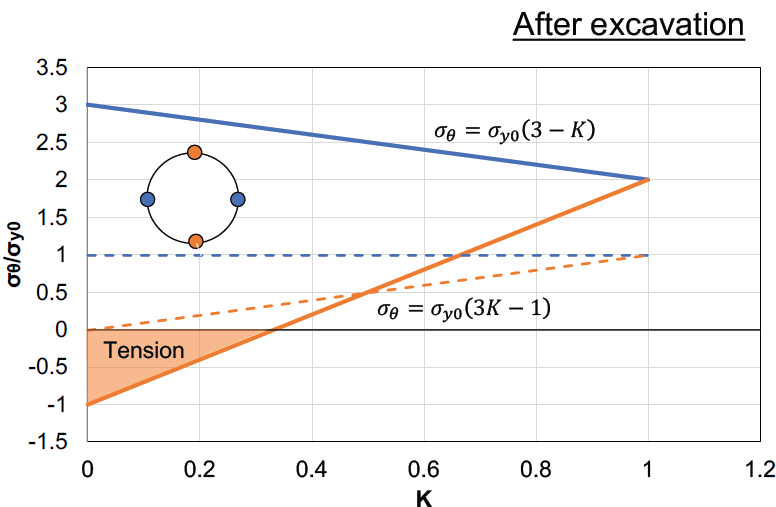
\includegraphics[width=0.15\textwidth]{stresses-boundary-circular-opening}
	\end{figure}
	
	\section{Stresses around a circular opening for $K=1$.}
	For an isotropic stress field ($K=1$), the Kirsch equations become
	\begin{align*}
		\sigma_r       & = \sigma_{y0}\left(1-\frac{R^2}{r^2}\right)+P\frac{R^2}{r^2} \\
		\sigma_\theta  & = \sigma_{y0}\left(1+\frac{R^2}{r^2}\right)-P\frac{R^2}{r^2} \\
		\tau_{r\theta} & = 0
	\end{align*}
	with $P$ an internal pressure.
	\begin{enumerate}[label=(\alph*)]
		\item When $P=\sigma_{y0}$, the internal pressure replaces the hydrostatic stress field present in the rock before excavation ($\sigma_r=\sigma_\theta=P$)
		\item By pressurizing the fluid in a borehole, it is possible to produce conditions where $P>\sigma_{y0}$ and, if $P>2\sigma_{y0}$, $\sigma_\theta$ will become negative (cf. hydraulic fracturing)
	\end{enumerate}
	
	\section{Induced displacement.}
	The magnitude of the displacements depends both on the natural stress field ($\sigma_{x0}$, $\sigma_{y0}$) and rock mass deformability ($G$, $v$).\\
	Radial displacement
	\[
		u_r = \frac{\sigma_{x0}+\sigma_{y0}}{4G}\frac{R^2}{r} + \frac{\sigma_{x0}-\sigma_{y0}}{4G}\frac{R^2}{r}\left[4(1-v)-\frac{R^2}{r^2}\right]\cos2\theta
	\]
	Orthoradial displacement
	\[
		u_\theta = -\frac{\sigma_{x0}-\sigma_{y0}}{4G}\frac{R^2}{r}\left[2(1-v)+\frac{R^2}{r^2}\right]\sin2\theta
	\]
	
	\section{Stress-controlled instabilities.}
	The Kirsch equations do not hold once the rock mass strength is reached (failure criterion) $\to$ stress-controlled instabilities.\\
	In \textbf{weak and soft} rock, the yielding may result in large convergence displacements (squeezing) where these displacements are a function of the size of the plastic zone relative to the tunnel diameter.
	In \textbf{hard and strong} rock, the yielding may result in relatively small convergence displacements as long as the depth of the brittle failure is limited and the bulking process in the failing rock is well controlled.\\
	The Kirsch solution can provide considerable insight into support design as it can be used to perform different types of preliminary investigations, such as  the determination of the zone influenced by an excavation and the identification of high stress regions where potential inelastic deformation may occur around excavations.\\
	Another type of stress-induced instability includes the possibility of \textbf{slip on pre-existing discontinuities} of the induced stress field.
	Slip on a pre-existing discontinuity will happen if the induced stresses locally satisfy the discontinuity shear strength criterion.\\
	Procedure:
	\begin{enumerate}
		\item Evaluate the stress components on the discontinuity using the Kirsch equations
		\item Transform these components into normal and shear stress components acting on the discontinuity
		\item Compare them to the discontinuity shear strength criterion
	\end{enumerate}
	
	\chapter{In situ stress.}
	
	Rocks differ from other materials in other fields because they are initially under stress.
	The state of stress in the subsurface prior to excavation is called the \textit{in situ} stress state.
	The in situ stress state influences the stability of underground and surface excavations.
	\begin{figure}[H]
		\centering
		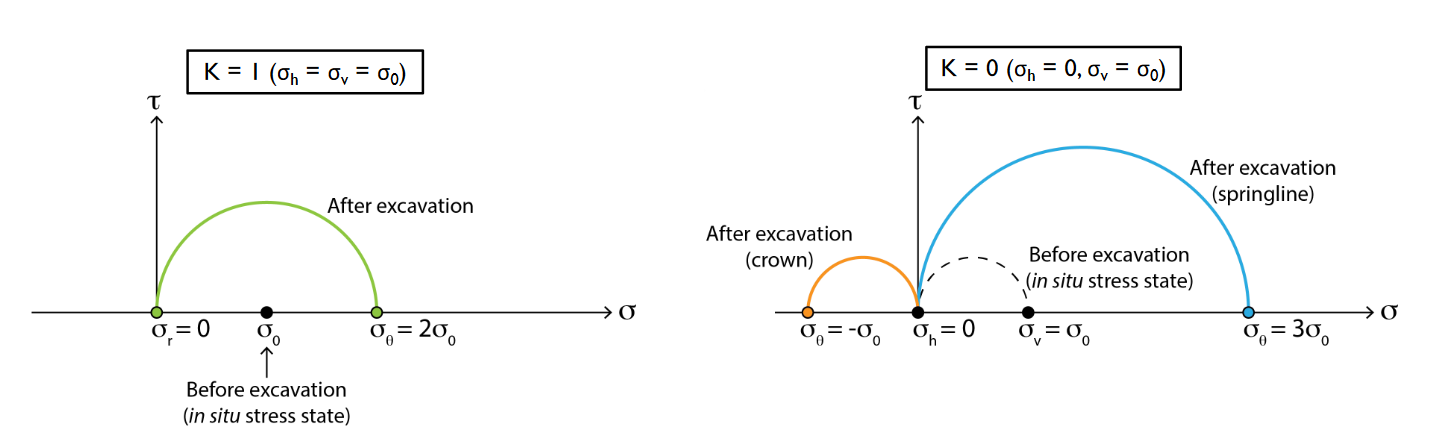
\includegraphics[width=0.35\textwidth]{in-situ}
	\end{figure}
	
	\section{Determining the stress state.}
	The state of stress at any point is defined with the stress tenor.
	Determining the stress state means determining the component of the stress tenor and determining the principal stress orientation.
	Any system utilised for estimating the in situ stress state must involve a minimum of \textbf{six} independent measurements.
	Direct stress measurement vs indirect methods/indicators.
	
	\section{In situ stress origins.}
	\begin{enumerate}
		\item \textbf{Lithostatic stress} from weight of overlying geological materials.\\
		      Horizontal stress
		      \[
			      \sigma_h=\sigma_H=K\sigma_v=\frac{\nu}{1-\nu}\sigma_v
		      \]
		      with $\nu\approx\SIrange{0.15}{0.35}{}$, $K\approx\SIrange{0.18}{0.54}{}$, and $\nu=-\varepsilon_r/\varepsilon_a$.\\
		      Vertical stress
		      \[
			      \sigma_v=\rho gz
		      \]
		      with $\rho g\approx\SI{0.027}{\mega\pascal\per\meter}$.
		\item \textbf{Tectonic stress} is responsible for the movement of lithospheric plates.
		      Stress state is in between active (normal faulting) and passive (reverse faulting) failure using Mohr Coulomb.
		      \begin{figure}[H]
			      \centering
			      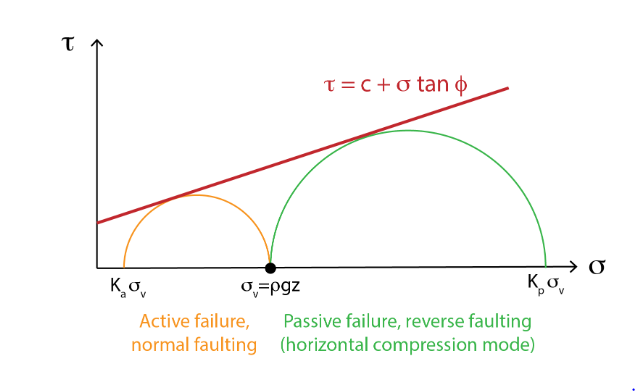
\includegraphics[width=0.25\textwidth]{tectonic-stress}
		      \end{figure}
	\end{enumerate}
	The mean worldwide horizontal stress does not follow the trend predicted by the elastic theory except at depths of several \SI{}{\kilo\meter}. For $0<z<\SI{500}{\meter}$, $\sigma_{H,\text{avg}}>\sigma_v$ for $90\%$ of cases.
	
	\section{In situ stress influences.}
	\begin{enumerate}
		\item \textbf{Surface topography}.
		      \begin{itemize}
			      \item Concave downward $\to$ large stress
			      \item Concave upward $\to$ low stress
			      \item Free surface with no stress acting on it $\to$ principal stress plane with zero normal stress
			      \item V-notch valley $\to$ very high horizontal \textit{in situ} stresses
		      \end{itemize}
		      The vertical direction is not always the principal stress direction.
		\item \textbf{Erosion.} When part of the overburden is eliminated from an area, the value of the vertical stress $\sigma_v$ is lowered and the state of stress and relationships between the acting stresses are modified.
		      \[
			      K(z)=K_0+\left[\left(K_0-\frac{\nu}{1-\nu}\right)\Delta z\right]\frac{1}{z}
		      \]
		\item \textbf{Fault and faulting}.
		\item \textbf{Intrusion.} Discontinuities: effect of stiffness of discontinuity filling material on stress state.
		      \begin{figure}[H]
			      \centering
			      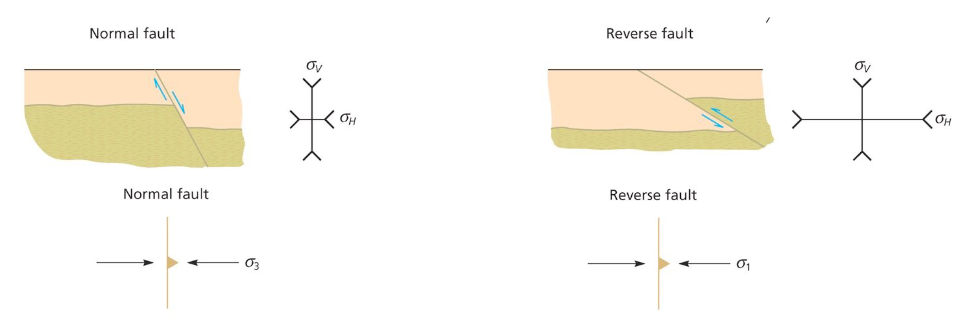
\includegraphics[width=0.34\textwidth]{fault-and-faulting}
		      \end{figure}
	\end{enumerate}
	
	\section{Hydraulic fracturing.}
	The objective of hydraulic fracturing is to measure at great depth ($>50\SI{}{\meter}$ and up to $\SI{5}{\kilo\meter}$) and through a borehole the magnitude and direction of the maximum and minimum principal stresses on a plane perpendicular to the borehole.\\
	The procedure consists of the following steps:
	\begin{enumerate}
		\item A length of borehole is chosen for the stress measurement, and an interval (typically $\SI{1}{\meter}$) is located for the test
		\item The interval is isolated using a packer system
		\item The isolated zone is pressurized by water until a fracture occurs in the rock
		\item Three measurements are taken:
		      \begin{itemize}
			      \item \textbf{Breakdown pressure} $P_f$: water pressure when the fracture occurs
			      \item \textbf{Shut-in pressure} $P_s$: subsequent pressure required to hold the fracture open
			      \item \textbf{Fracture re-opening pressure} $P_r$: pressure required to re-open the fracture
		      \end{itemize}
	\end{enumerate}
	Assumes that a vertical borehole is drilled in a non-porous, impermeable formation and the three principal stresses are the vertical stress $\sigma_v$ and the horizontal stresses $\sigma_H$ and $\sigma_h$ with $\sigma_H>\sigma_h$.
	Kirsch analytical solution in slides.
	Initially $\sigma_\theta(A)=3\theta_h-\sigma_H$.
	\begin{enumerate}
		\item The fluid is pumped to the borehole section insulated by the two packers $\to$ the fluid pressure in the borehole increases:
		      \[
			      \sigma_\theta(A)=3\sigma_h-\sigma_H-P
		      \]
		\item More fluid is injected in the borehole section insulated by the two packers $\to$ the borehole pressure reaches the rock fracturing pressure $\to$ the fracture initiates:
		      \[
			      \sigma_\theta(A)=3\sigma_h-\sigma_H-P_f=-T_0
		      \]
		      $\to$ the fracture propagates in the direction perpendicular to the minimum \textit{in situ} stress (assumption) but the fluid pressure in the fracture drops.
		\item When the fluid pressure equals $\sigma_h$, the fracture cannot propagate further and closes. The shut-in pressure is such that
		      \[
			      P=P_s=\sigma_h
		      \]
		\item The fluid pressure is increased again to re-open the fracture:
		      \[
			      \sigma_\theta(A)=3\sigma_h-\sigma_H-P_r=0
		      \]
	\end{enumerate}
	Derived from the equations above:
	\begin{align*}
		\sigma_h=P_s  \\
		(P_f-P_r)=T_0 \\
		\sigma_H=3\sigma_h-P_r
	\end{align*}
	
	\section{Flat jack.}
	\begin{enumerate}
		\item Two pins are drilled and fixed into an excavation boundary. The distance between them is denoted $\text{d}_0$.
		\item A slot is cut into the rock halfway between the pins.
		\item As the rock is cut, the pins will move together (if the normal stress is compressive).
		\item A flat jack is grouted in the slot.
		\item The flat jack is pressurised with oil or water.
		\item The pins move apart.
	\end{enumerate}
	The flat jack is said to be a self-compensating method of stress determination.
	\textbf{One} normal stress component across the flat-jack can be determined using the flat jack method.
	\textbf{Six} tests with different independent orientations and locations are needed to fully characterise the \textit{in situ} state of stress.
	\begin{figure}[H]
		\centering
		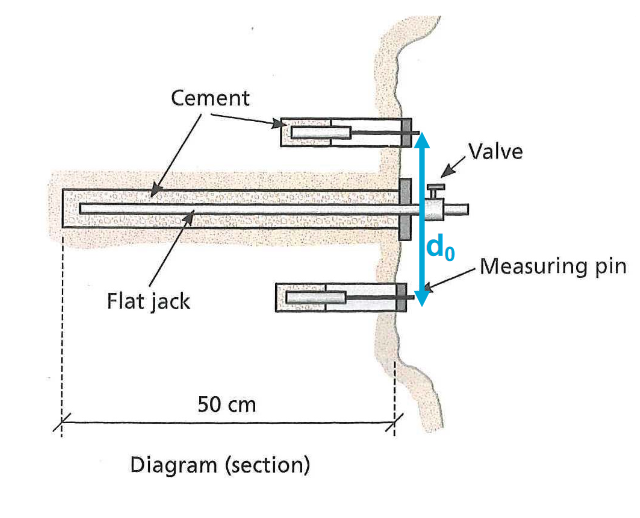
\includegraphics[width=0.2\textwidth]{flat-jack}
	\end{figure}
	In practice: performed at a rock face; pressures until \SI{34.5}{\mega\pascal} (if careful welding); $\text{d}_0$ is typically six inches (\SI{15.2}{\centi\meter}).
	
	\chapter{Discontinuities characterisation and behaviour.}
	
	\section{Impact of discontinuities on rock masses.}
	\textbf{Tunnels}.
	Influences of the pre-existing discontinuities on the nucleation of new creaks --- weakness zone.
	Effect: blocks might fall from the roof of a tunnel due to intersecting joint planes; at a larger scale, whole chambers can collapse owing to unfortunate intersections of planar weaknesses.\\
	\textbf{Slopes}.
	Influence of the pre-existing discontinuities and of the slope on unstable block of rocks (toppling).
	Effects: column of rocks rotates at the base of the slope and falls; toppling failure occurs in nature but also in mining excavation where the confining stresses are reduced.
	
	\section{Basic characteristics of discontinuities.}
	A discontinuity is a planar structure in the rock.
	Structural discontinuities occur at different scales and in different contexts.\\
	Geometric attributes of discontinuity systems:
	\begin{itemize}
		\item Discontinuity orientation and sets
		\item Persistence
		\item Spacing and block sizes
		\item Roughness and aperture
	\end{itemize}
	
	\section{Discontinuity orientations and sets.}
	\textbf{Characterisation}.
	Orientation of discontinuities controls the possibility of unstable conditions or excessive deformations.
	The orientation of discontinuities determine the shape of rock blocks.
	The orientation is defined by the direction of the plane (strike) and its dip.\\
	\textbf{Notation}.
	Discontinuities are organised in networks composed of one or more sets.
	Sets are generally defined based on their orientations.
	The most common networks are orthogonal, conjugated, hexagonal, and polygonal --- best way to observe them is in outcrops.\\
	\textbf{Characterising sets.}
	Mechanical properties of the rock mass are influenced by discontinuities sets. More sets = more possibilities for potential slide planes.
	One set cuts the rock into planes, two orthogonal sets into columns, and three into blocks.\\
	ISRM suggested classification:
	\begin{table}[H]\scriptsize\centering\begin{tabular}{ll}
			%				\hline
			I    & Massive, occasional random fractures   \\
			%				\hline
			II   & One joint set                          \\
			%				\hline
			III  & One joint set plus random fractures    \\
			%				\hline
			IV   & Two joint sets                         \\
			%				\hline
			V    & Two joint sets plus random fractures   \\
			%				\hline
			VI   & Three joint sets                       \\
			%				\hline
			VII  & Three joint sets plus random fractures \\
			%				\hline
			VIII & Four or more joint sets                \\
			%				\hline
			IX   & Crushed rock, earth-like               \\
			%				\hline
		\end{tabular}\end{table}
	
	\section{Persistence, spacing, and block size.}
	\textbf{Persistence}.
	The persistence is the areal extent of a rock discontinuity.
	The persistence of sets of discontinuities controls large-scale rock or structural failure.
	\begin{table}[H]\scriptsize\centering\begin{tabular}{ll}
			%				\hline
			ISRM Suggested Description & Surface Trace Length (\SI{}{\meter}) \\
			\hline
			Very low persistence       & $<1$                                 \\
			%				\hline
			Low persistence            & \SIrange{1}{3}{}                     \\
			%				\hline
			Medium persistence         & \SIrange{3}{10}{}                    \\
			%				\hline
			High persistence           & \SIrange{10}{20}{}                   \\
			%				\hline
			Very high persistence      & $>20$                                \\
			%				\hline
		\end{tabular}\end{table}
	\textbf{Spacing}.
	The fracturing degree of a rock mass is controlled by the number of discontinuities in the rock mass.
	More discontinuities implies a decrease of the spacing.
	Discontinuity spacing controls the size of individual rock blocks (failing mode).
	Discontinuity spacing is the orthogonal distance between two consecutive discontinuities.\\
	\textbf{Frequency/density of discontinuities}.
	Discontinuity frequency $\lambda$ is the number of discontinuity per unit length (i.e. inverse of joint spacing $s_j$):
	\[
		\lambda=\frac{1}{s_j}
	\]
	The frequency is linked with the density of fracturing.
	\begin{table}[H]\scriptsize\centering\begin{tabular}{ll}
			%				\hline
			Description             & Joint Spacing (\SI{}{\meter}) \\
			\hline
			Extremely close spacing & $<0.02$                       \\
			%				\hline
			Very close spacing      & \SIrange{0.02}{0.06}{}        \\
			%				\hline
			Close spacing           & \SIrange{0.06}{0.2}{}         \\
			%				\hline
			Moderate spacing        & \SIrange{0.2}{0.6}{}          \\
			%				\hline
			Wide spacing            & \SIrange{0.6}{2}{}            \\
			%				\hline
			Very wide spacing       & \SIrange{2}{6}{}              \\
			%				\hline
			Extremely wide spacing  & $>6$                          \\
			%				\hline
		\end{tabular}\end{table}
	\textbf{Rock quality designation}.
	Expresses the percentage of segments of intact rocks of more than \SI{10}{\centi\meter} long ($L_i$) over the considered length ($L$):
	\[
		\text{RQD}=\frac{\sum{L_i}}{L}\cdot100\%,\quad L_i>\SI{10}{\centi\meter}
	\]
	\begin{table}[H]\scriptsize\centering\begin{tabular}{ll}
			%					\hline
			Very poor  & \SIrange{0}{25}{\percent}   \\
			%					\hline
			Poor       & \SIrange{25}{50}{\percent}  \\
			%					\hline
			Fair       & \SIrange{50}{75}{\percent}  \\
			%					\hline
			Good       & \SIrange{75}{90}{\percent}  \\
			%					\hline
			Excellence & \SIrange{90}{100}{\percent} \\
			%					\hline
		\end{tabular}\end{table}
	
	\section{Roughness.}
	Defines the morphology of discontinuity walls.
	Varies from smooth to very rough.
	Walls can be in contact and matched or poorly linked and mismatched.
	The roughness controls the resistance to present-day shear stress: very rough surfaces in good contact will be much more difficult to displace than smooth ones.\\
	Discontinuity surface roughness is a measure of surface unevenness and waviness relative to its mean plane.
	The roughness is characterised by large-scale waviness (undulation) and small-scale unevenness (irregularity) of a discontinuity surface.
	The roughness principal governing factor of the direction of hear displacement and shear strength, in turn, the stability of potentially sliding blocks.\\
	Should first be described qualitatively at metre scale (step, undulating, planar) and then at centimetre scale (rough, smooth, slickensided).
	Joint Roughness Coefficient (JRC) is a quantitative measure of roughness, varying from $0$ for the smooth flat surface to $20$ for the very rough surface.
	
	\section{Aperture.}
	In a natural joint, it is very seldom that the two surfaces are in complete contact.
	The perpendicular distance separating the adjacent rock walls is termed as aperture.
	Joint opening is either filled with air and water (open joint) or with infill materials (filled joint).
	Joints with large apertures have low shear strength.
	Aperture associates with flow and permeability.
	\begin{table}[H]\scriptsize\centering\begin{tabular}{lll}
			Aperture                          & Description           &                 \\
			\hline
			$<\SI{0.1}{\milli\meter}$         & Very tight            &                 \\
			\SIrange{0.1}{0.25}{\milli\meter} & Tight                 & Closed fracture \\
			\SIrange{0.25}{0.5}{\milli\meter} & Partly open           &                 \\
			\hline
			\SIrange{0.5}{2.5}{\milli\meter}  & Open                  & Gapped          \\
			\SIrange{2.5}{10}{\milli\meter}   & Widely open           & feature         \\
			\hline
			\SIrange{1}{10}{\centi\meter}     & Very widely open      &                 \\
			\SIrange{10}{100}{\centi\meter}   & Extremely widely open & Open feature    \\
			$>\SI{1}{\meter}$                 & Cavernous             & 
		\end{tabular}\end{table}
	Can be expressed as a function of length but also as a function of reactivation from present day \textit{in situ} stress.
	Aperture can be the real aperture or the equivalent hydraulic aperture.\\
	Filling is material in the rock discontinuities separating the adjacent rock surfaces.
	Filled discontinuity is the only way of evaluating real aperture occurring in subsurface condition.
	In general, properties of the filling material affect shear strength, deformability, and permeability of the discontinuities.
	
	\section{Key mechanical properties.}
	Previously we discussed the mechanical behaviour of intact rock via the stress-strain curve.
	Here, consider the equivalent behaviour of a discontinuity loaded in compression and/or shear.
	\begin{align*}
		\text{Normal stress}\        & \sigma_n=\frac{N}{A} \\
		\text{Normal displacement}\  & \Delta n             \\
		\text{Shear stress}\         & \tau=\frac{T}{A}     \\
		\text{Shear displacement}\   & \Delta s
	\end{align*}
	\begin{figure}[H]
		\centering
		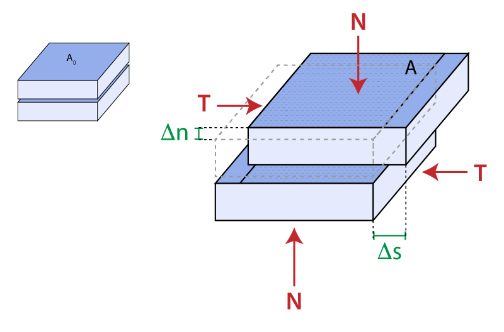
\includegraphics[width=0.2\textwidth]{direct-shear-test}
	\end{figure}
	
	\section{Shear strength of rock joints.}
	Conditions for sliding of rock blocks along existing joints and faults at slope or excavation opening are governed by the shear stress developed on the sliding rock discontinuities and shear strength.
	For a test carried out at a constant normal stress, a typical plot of the shear stress against the shear displacement is
	\begin{figure}[H]
		\centering
		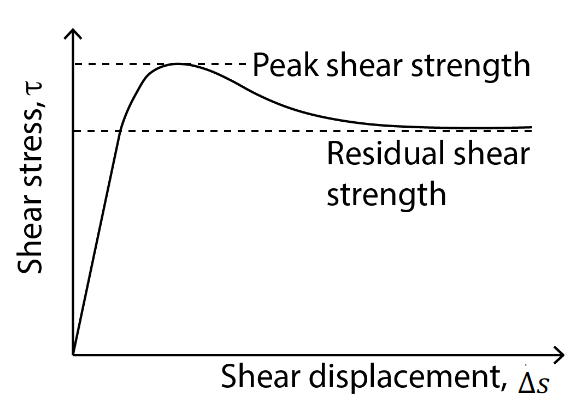
\includegraphics[width=0.17\textwidth]{shear-stress-displacement}
	\end{figure}
	At small displacements, the specimen behaves elastically and the shear stress increases linearly with displacement.
	As the force resisting movement is overcome, the curve becomes non-linear and then reaches a maximum that represents the peak shear strength of the discontinuity.
	Thereafter, the stress required to cause displacement decreases and eventually reaches a constant value termed the residual shear strength.
	
	\section{Friction angle of rock surfaces.}
	For a planar, clean (no infilling) discontinuity, the cohesion will be zero and the shear strength will be defined solely by the friction angle.
	The basic friction angle of the rock material is related to the size and shape of the grains exposed on the fracture surface
	\begin{itemize}
		\item Fine-grained rock and rock with a high mica content will tend to have a low friction angle
		\item Coarse-grained rock will have a high friction angle
	\end{itemize}
	\begin{table}[H]\scriptsize\centering\begin{tabular}{lll}
			Rock class      & Friction angle              & Typical rock types                         \\
			\hline
			Low friction    & $\SIrange{20}{27}{\degree}$ & Schists (high mica content), shale, marl   \\
			Medium friction & $\SIrange{27}{34}{\degree}$ & Sandstone, siltstone, chalk, gneiss, slate \\
			High friction   & $\SIrange{34}{40}{\degree}$ & Basalt, granite, limestone, conglomerate
		\end{tabular}\end{table}
	
	\section{Shearing on an inclined plane.}
	If the discontinuity surface is inclined at an angle $i$ to the shear stress direction, the shear and normal stresses acting on the sliding surface are given by
	\begin{align*}
		\tau_i   & =\tau\cos^2i-\sigma\sin i\cos i \\
		\sigma_i & =\sigma\cos^2i+\tau\sin i\cos i
	\end{align*}
	If it is assumed that the discontinuity surface has zero cohesion and that its shear strength is $\tau_i=\sigma_i\tan\phi$, then
	\[
		\tau=\sigma\tan(\phi+i)
	\]
	where $\phi$ is the basic friction angle and $(\phi+i)$ is the apparent friction angle.
	\begin{figure}[H]
		\centering
		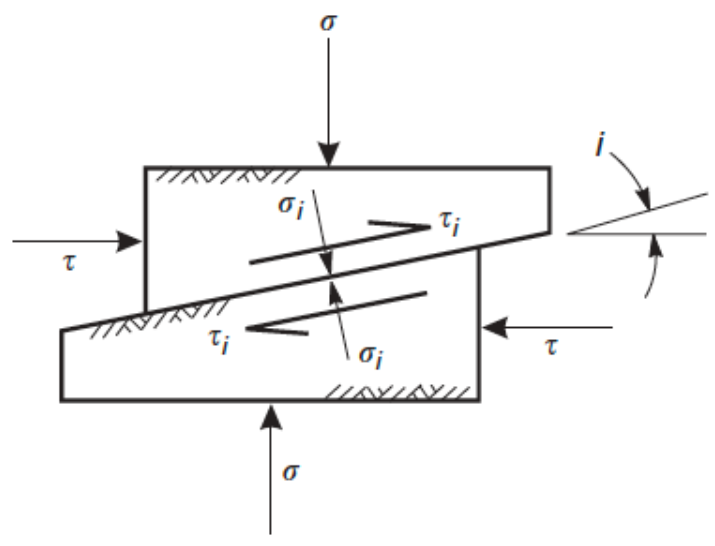
\includegraphics[width=0.15\textwidth]{shearing-inclined-plane}
	\end{figure}
	
	\section{Effect of surface roughness.}
	The same equation is valid for a rough discontinuity with an average asperity inclination $i$:
	\[
		\tau=\sigma\tan(\phi+1)
	\]
	The dilation (normal displacement $\Delta n$) due to the shear displacement $\Delta s$ is given by
	\[
		\Delta n=\Delta s\tan i
	\]
	\begin{figure}[H]
		\centering
		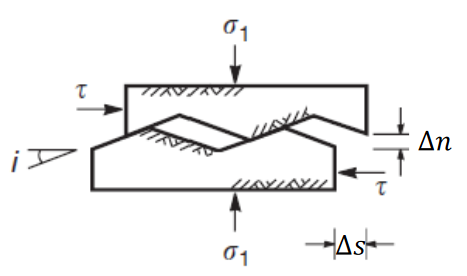
\includegraphics[width=0.15\textwidth]{surface-roughness}
	\end{figure}
	For higher levels of normal stress, the shear displacement will shear off asperities, with consequent reduction of the effective friction angle and of the normal dilation.
	In the limit, as normal stress approaches the joint compressive strength, the effective friction angle tends to the basic friction angle.
	
	\section{Shear strength model I: Mohr-Coulomb.}
	We obtain a residual failure envelope with the residual shear strength.
	Cohesion disappears in the residual state.
	Stress states in the blue zone are not possible in the residual strength condition.
	\begin{figure}[H]
		\centering
		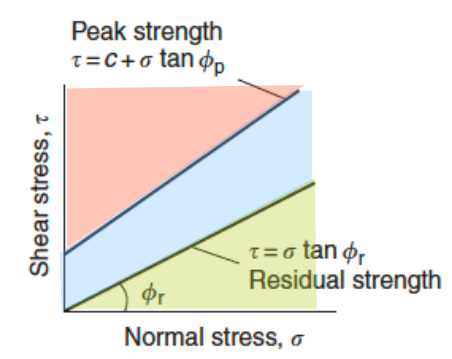
\includegraphics[width=0.15\textwidth]{residual-failure-envelope}
	\end{figure}
	with peak friction angle $\phi_p$, residual friction angle $\phi_r$, and cohesion of the cementing material $c$.
	
	\section{Shear strength model II: bi-linear model.}
	Shear strength for a rough fracture could exhibit two features: at low normal stress shearing by climbing the asperity angle; at high stress shearing off the asperities.
	This leads to a bilinear shear strength model
	\begin{align*}
		\tau & =\sigma_n\tan(\phi+1) & \ \text{for} \ \sigma_n\leq\sigma_n^\ast \\
		\tau & =c+\sigma_n\tan(\phi) & \ \text{for} \ \sigma_n\geq\sigma_n^\ast
	\end{align*}
	where $\sigma_n^\ast$ is the critical normal stress when shearing of asperity is assumed to start.
	
	\section{Shear strength model III: JRC-JCS empirical model.}
	In reality, there is no clear boundary between shearing by climbing asperity and shearing off asperities.
	The actual shear stress-normal stress relation is represented by a curve, and could be represented by the empirical relation
	\[
		\tau=\sigma_n\tan\left[\text{JRC}\log_{10}\left(\frac{\text{JCS}}{\sigma_n}\right)+\phi_r\right]
	\]
	with effective normal stress $\sigma_n$, joint roughness coefficient JRC, joint wall compressive strength JCS, and drained residual friction angle $\phi_r$.
	Comments: it has the basic form of friction law; high JRC gives high dilation angle ($i$); higher JCS delays the reduction of $i$, since strong rock has less shearing off; it is widely accepted and used in rock engineering.
	
	\section{Peak shear strength modes.}
	Joint surface profile is a 3D feature, while shearing is a directional activity.
	Surface profile along a particular direction would be different along another direction and hence gives different shear strength.
	
	\section{Water and rock joint shear strength.}
	When a joint is wet, it has generally a lower friction angle than a dry joint.
	When shear strength of a wet joint is calculated, use the wet (and drained) friction angle.
	If a joint is submerged to water pressure, normal stress is the shear strength equation is the effective normal stress.
	\[
		\tau=c+(\sigma_n-p_w)\tan(\phi+i)
	\]
	
	\section{Stereographic projections.}
	%		The orientation of a plane (discontinuity) can be represented using stereological projection methods.
	%		The projection method allows three-dimensional orientation data to be represented and manipulated.
	%		The stereographic projection is essential to quickly interpret patterns of preferred orientations.
	\begin{enumerate}
		\item A line or a plane is measured into an outcrop.
		\item Include the discontinuity at the centre of a sphere. The line or the plane is, by convention, localised in the lower hemisphere.
		\item For a line, the point of intersection with the sphere envelope is called the spherical projection of the line. For a plane, the intersection with the sphere envelope is the great circle.
		\item If we had the sphere in front of us, the structural line is a point in the lower hemisphere and a plane is a great circle.
		\item Project lines and plane on the equatorial plane or plane of projection. Any point on the lower hemisphere projects a dot on the plane of projection and a great circle becomes a circular arc.
	\end{enumerate}
	\begin{figure}[H]
		\centering
		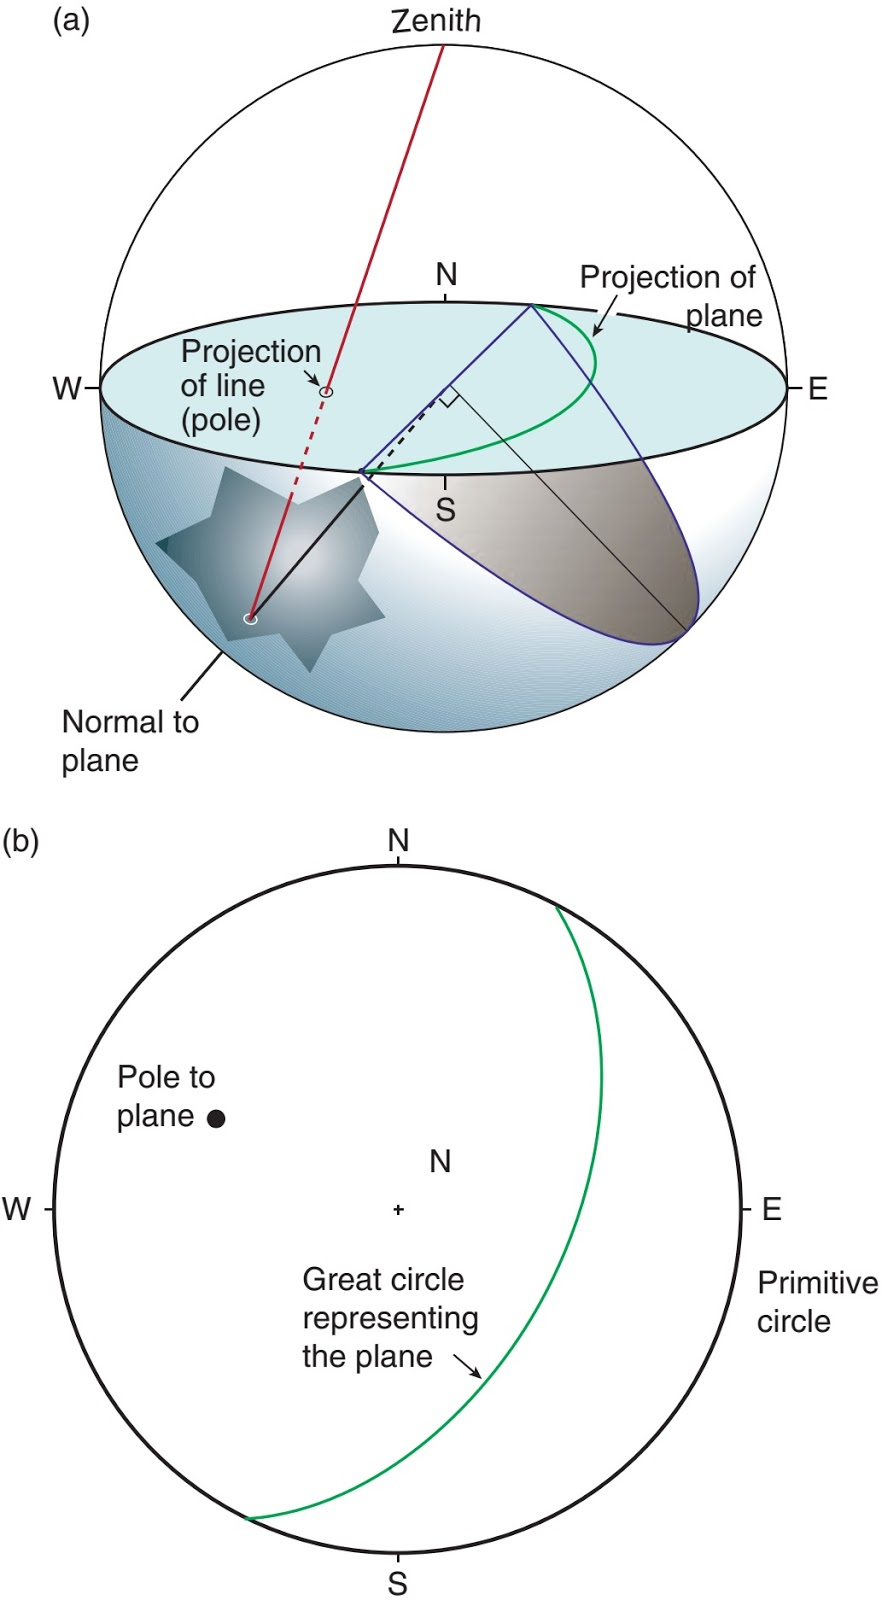
\includegraphics[width=0.13\textwidth]{stereographic}
	\end{figure}
	
	\chapter{Surface excavations.}
	
	Needed when linear infrastructure or mining requires the construction of either a level surface on natural slopes or a pre-determined depth below ground level.
	Slope stability is determined by
	\begin{itemize}
		\item Geometric factors (height, angle, orientation)
		\item Geological factors (discontinuities, anisotropy)
		\item Hydrogeological factors (water, permeability)
		\item Geomechanical factors (strength, deformability and permeability)
	\end{itemize}
	
	\section{Modes of failure.}
	Different types of rock slope failure are conditioned by
	\begin{itemize}
		\item The characteristics of the rock mass (number of joint sets, orientation of the discontinuities, characteristics of the discontinuities...)
		\item The orientation of the slope face with respect to the orientation and distribution of the discontinuities
	\end{itemize}
	The stability is defined by the strength of the discontinuities and the intact rock
	\begin{itemize}
		\item In hard or strong rock masses, the location of the failure planes is determined by the discontinuities
		\item In weak rock masses, intact rock also plays an important part in the development and location of such planes and in the failure mechanism
	\end{itemize}
	\begin{figure}[H]
		\centering
		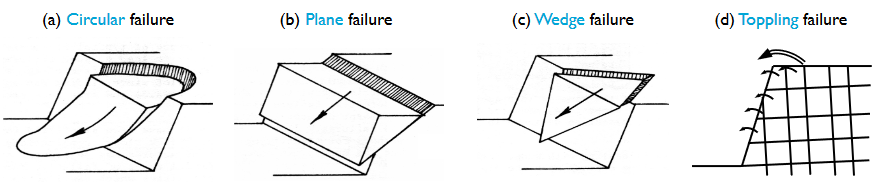
\includegraphics[width=0.3\textwidth]{modes-of-failure}
	\end{figure}
	\subsection{(a) Circular failure.}
	Usually occurs in waste rock, heavily fractured rock, and weak rock with no identifiable structural pattern.
	The failure surface is free to find a line of least resistance through the slope.
	The crushed or highly fractured rock masses are assumed to be homogeneous, and the shear strengths are controlled by cohesion and friction.
	Circular failure analysis: analytical methods as in soil mechanics; $c$ and $\phi$ are for rock mass.
	\subsection{(b) Plane failure.}
	Occurs in rocks with plane discontinuities, e.g. bedding planes.
	Necessary criteria for kinematic feasibility:
	\begin{enumerate}
		\item The potential sliding plane dips out of the slope
		\item The dip of the slope must exceed that of the potential slide plane
		\item The dip of the potential slide plane is such that the strength of the plane is reached
	\end{enumerate}
	\subsection{(c) Wedge failure.}
	Occurs when two planes of weakness intersect to define a tetrahedral block.
	Necessary criteria for the kinematic feasibility:
	\begin{enumerate}
		\item The potential intersection line must dip out of the slope
		\item The dip of the slope must exceed that of the potential slide line
		\item The dip of the potential slide line is such that the strength of the line is reached
	\end{enumerate}
	\subsection{(d) Toppling failure.}
	Occurs in rocks with columnar or block structures separated by steeply dipping discontinuities.
	Two types of toppling failure
	\begin{itemize}
		\item Direct toppling: if there are frequent cross joints, the layers can overturn as rigid columns
		\item Flexural toppling: each layer tending to bend down-hill under its own weight transfers force downslope. If the toe of the slope is allowed to slide, flexural cracks will form in the layers above, liberating a large mass of rock
	\end{itemize}
	
	\section{Stability analysis.}
	The analysis of rock slope stability is fundamentally dependent on a detailed analysis of the rock mass structure.
	A kinematic analysis is then performed to determine the influence of the discontinuities on stability and identify possible modes of slope failure.
	Involves studying the relationship between the orientation of the discontinuity and the face.
	
	\section{Limit equilibrium analysis.}
	Calculates the factor of safety of the slope.
	The forces tending towards movement along a given failure surface are compared with the forces resisting it.
	The Factor of Safety (FoS) is defined as
	\[
		\text{FoS}=\frac{\text{Forces resisting slide}}{\text{Forces tending to slide}}=\frac{\sum R}{\sum S}=\frac{\text{Resisting shear stress}}{\text{Sliding shear stress}}
	\]
	The slope is stable if $\text{FoS}>1$.
	\begin{enumerate}
		\item Section of potential sliding surface(s)
		\item Triggering and resisting forces
		\item Mohr-Coulomb failure criterion
		\item Definition of factor of safety (FoS)
	\end{enumerate}
	\begin{figure}[H]
		\centering
		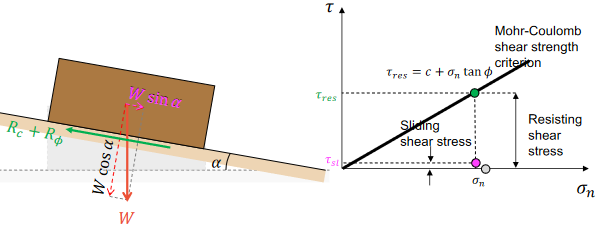
\includegraphics[width=0.25\textwidth]{limit-equilibrium-analysis}
	\end{figure}
	\begin{align*}
		\text{FoS} & =\frac{\tau_\text{res}}{\tau_\text{sl}}=\frac{c+\frac{W\cos\alpha}{A}\tan\phi}{\frac{W\sin\alpha}{A}}=\frac{cA+W\cos\alpha\tan\phi}{W\sin\alpha} \\
		           & =\frac{R_c+R_\phi}{W\sin\alpha}
	\end{align*}
	\[
		\sigma_n=\frac{W\cos\alpha}{A}\quad\tau_\text{sl}=\frac{W\sin\alpha}{A}\quad\tau=c+\sigma_n\tan\phi
	\]
	Limit-equilibrium analysis is based on
	\begin{itemize}
		\item Section of potential sliding surface(s)
		\item Mohr-Coulomb failure criterion
		\item Definition of FoS
		      \begin{enumerate}
			      \item Identification of all forces acting on the sliding mass
			      \item Calculation of the resultant resisting and driving forces
			      \item Calculation of the FoS
		      \end{enumerate}
	\end{itemize}
	
	\section{Slope stabilisation measures.}
	%		The following issues must be considered when selecting a stabilisation measure:
	%		\begin{itemize}
	%			\item Geotechnical conditions (geology, rock strength, groundwater, failure mechanism, dimensions of the instability)
	%			\item Construction (optimum level of work, costs, equipment access, available work time during traffic closures, disposal of waste rock and soil)
	%			\item Aesthetics
	%			\item Environment
	%		\end{itemize}
	Five general categories of slope stabilisation measures:
	\begin{enumerate}
		\item Change of the slope geometry
		      \begin{itemize}
			      \item Modifying the slope geometry redistributes forces due to the weight of the materials to obtain a more stable configuration
			      \item It may include reducing the slope angle, removing weight at the head of the slope, increasing weight at the slope toe, constructing benches and berms (stepping)
			      \item Rock removal should only be used where it is certain that the new face will be stable, and there is no risk of undermining the upper part of the slope
		      \end{itemize}
		\item Mechanical stabilisation
		      \begin{itemize}
			      \item Mechanical methods of slope stabilisation are those that alter or protect the slope face to reduce erosion, prevent rock fall, or to reduce ravelling
			      \item Common methods include protective blankets, geotextiles, and wire nets/meshes
		      \end{itemize}
		\item Structural stabilisation
		      \begin{itemize}
			      \item Structural stabilisation includes those methods that reinforce the structure of the rock at the slope face or provide a structure that supports the slope
			      \item Methods available include the use of gunite or shotcrete, the use of rock bolting, the construction of rock buttresses, and the construction of retaining walls
		      \end{itemize}
		      Pre-tensioned rock bolt
		      \[
			      \text{FoS}=\frac{\left[W\cos\alpha+T\sin(\alpha+\beta)\right]\cdot\tan\phi}{W\sin\alpha-T\cos(\alpha+\beta)}
		      \]
		      Pre-tensioned net
		      \[
			      \text{FoS}=\frac{\left[W\cos\alpha+p\cdot A\right]\cdot\phi}{W\sin\alpha}
		      \]
		\item Vegetative stabilisation
		      \begin{itemize}
			      \item Most frequently used for aesthetic purposes, such as slope reclamation
			      \item Generally, these methods are most successful when minor or shallow instability (such as ravelling or erosion) is involved, as is usually the case for soil slopes or highly fractured rock slopes
		      \end{itemize}
		\item Water control
		      \begin{itemize}
			      \item Groundwater in rock slopes is often a primary or contributory cause of instability: reduction of the shear strength of the potential failure surface; accelerate weathering; expansion of openings when freezing; erosion
			      \item A reduction in water pressures usually improves stability
			      \item Drainage can be at ground level (drainage ditches, channels...) or at depth (horizontal drains, wells, drainage walls...)
		      \end{itemize}
	\end{enumerate}
	
	\newpage
\end{multicols}
\end{document}
